%--------------------
% Packages
% -------------------
\documentclass[11pt,a4paper]{article}

\usepackage[utf8x]{inputenc}
\usepackage[T1]{fontenc}
\usepackage{mathptmx} % Use Times Font
\usepackage[pdftex]{graphicx} % Required for including pictures
% \usepackage[pdftex,linkcolor=black,pdfborder={0 0 0}]{hyperref} % Format links for pdf
\usepackage{calc} % To reset the counter in the document after title page
\usepackage{enumitem} % Includes lists
\usepackage{csquotes} % Exercise as quotes
\usepackage{amsmath} % For using "equation*" 
\usepackage{nicefrac} % For in-line fractions

\setcounter{equation}{0}% How to reset equation counter

\frenchspacing % No double spacing between sentences
\linespread{1.2} % Set linespace
\usepackage[a4paper, lmargin=0.1666\paperwidth, rmargin=0.1666\paperwidth, tmargin=0.1111\paperheight, bmargin=0.1111\paperheight]{geometry} %margins
%\usepackage{parskip}

\usepackage[all]{nowidow} % Tries to remove widows
\usepackage[protrusion=true,expansion=true]{microtype} % Improves typography, load after fontpackage is selected
%-----------------------
% Set pdf information and add title, fill in the fields
%-----------------------
% \hypersetup{ 	
% pdfsubject = {Nano-Optics},
% pdftitle = {Assignment 1},
% pdfauthor = {Vlad Tkachuk}
% }

%-----------------------
% Begin document
%-----------------------
\begin{document} 

\section{Theory}
\subsection*{Exercise 1}
You have fabricated a photonic crystal having the following 2-D triangular lattice (Figure~\ref{fig:fig0}):

\begin{figure}[ht]
   \centering
    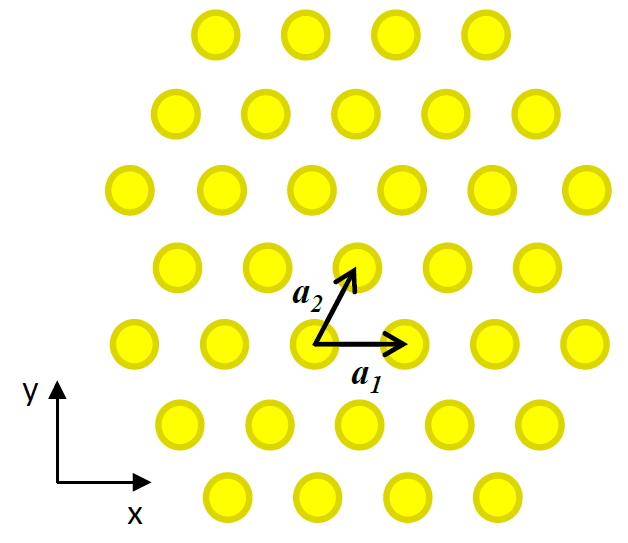
\includegraphics[width=0.45\textwidth]{fig0.png}
    \caption{Real space lattice of a triangular 2-D photonic crystal in silicon.}
    \label{fig:fig0}
\end{figure}


Each of the yellow rods is made of silicon and the surrounding material is air. For this structure:

\begin{displayquote}
\textbf{1.} Give the expressions of both the real and reciprocal lattice primitive vectors in the Cartesian coordinate system ($\hat{x}, \; \hat{y}$).
\end{displayquote}

Figure 1 suggests a equilateral triangle arrangement, such that $|\vec{a_1}|=|\vec{a_2}|=a$. This implies that the angle between the vectors is $\nicefrac{\pi}{3}$. If we align $\vec{a_1}$ with x-axis then $\vec{a_1}=a\hat{x}$. We can readily obtain decomposition of $\vec{a_2}=a\frac{1}{2}\hat{x}+a\frac{\sqrt{3}}{2}\hat{y}$. The simplest way of calculation would be using quasi-3D lattice in which $\vec{a_3}=\hat{z}$.  Then we can use the vector multiplication shortcut formulas to obtain the reciprocal lattice:

\begin{equation*}
    b_1=2\pi \frac{a_2\times a_3}{a_1 \cdot(a_2 \times a_3)}= \frac{2 \pi}{a} \hat{x} -\frac{2\sqrt{3}\pi}{3a} \hat{y} 
\end{equation*}

\begin{equation*}
    b_2=2\pi \frac{a_3\times a_1}{a_1 \cdot(a_2 \times a_3)}= \frac{4\sqrt{3}\pi}{3a} \hat{y} 
\end{equation*}

\begin{equation*}
    b_3=2\pi \frac{a_1\times a_2}{a_1 \cdot(a_2 \times a_3)}= 2 \pi 
\end{equation*}

\begin{displayquote}
\textbf{2.} Draw the reciprocal lattice. Draw the Brillouin zone and the reduced Brillouin zone.
\end{displayquote}
See Figure~\ref{fig:fig2}.
\begin{figure}[ht]
   \centering
    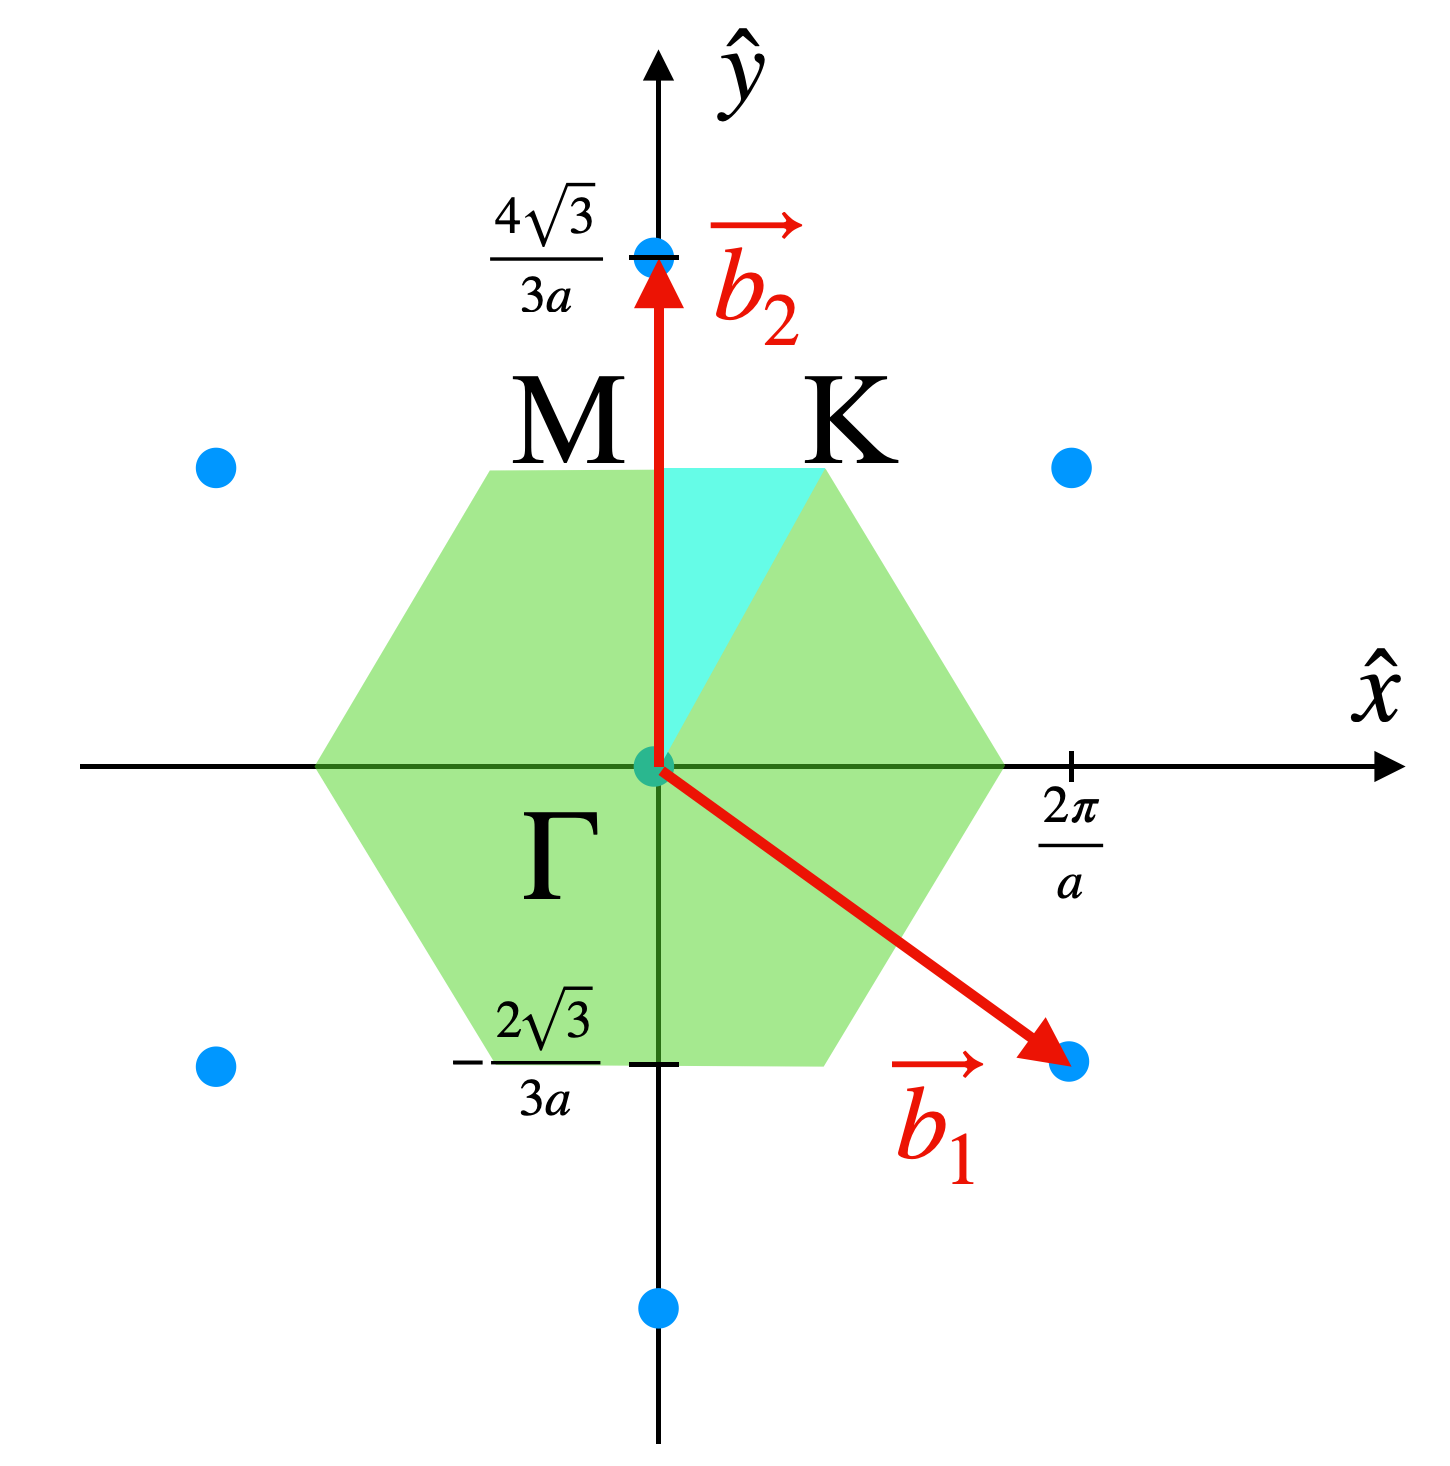
\includegraphics[width=0.45\textwidth]{fig2.png}
    \caption{Reciprocal lattice of the triangular lattice from Figure 1, Brillouin zone (green) and reduced Brillouin zone (blue).}
    \label{fig:fig2}
\end{figure}

\begin{displayquote}
\textbf{3.} You need to calculate the bandstructure of the photonic crystal described in Fig.1. What is the “bandstructure”? What information can you obtain from the bandstructure?
\end{displayquote}

Band structure is a family of dispersion relations for different modes in a photonic crystal. From it we can see wavevectors for different frequencies and polarizations. There could be a photonic bandgap where no wavevectors are allowed to propagate in range of frequencies. Around these frequencies we can see positive, null and negative group velocity regions. 

\begin{displayquote}
\textbf{4.} Explain how would you calculate the band structure using the Bloch theorem. Over which range of k-vectors should you calculate the $\omega_k$? Why?
\end{displayquote}
Bloch theorem postulates that the field in the periodic structure can be expressed as:
\begin{equation*}
    \vec{H}(\vec{r}) = e^{i \vec{k}\cdot \vec{r}} \cdot \vec{u} (\vec{r})
\end{equation*}
i.e. as product of plane wave function and periodicity function. 
To calculate the band structure, we solve the master equation for eigenfuncitons:
\begin{equation*}
    \nabla \times \bigg(\frac{1}{\varepsilon(\vec{r})}\nabla \times\vec{H}({\vec{r}}) \bigg)=\mu_0 \varepsilon_0 \omega_n^2(\vec{k}) \vec{H} (\vec{r})
\end{equation*}
The range of wavevectors is defined by the irreducible Brillouin zone and its symmetry points, in our case, $\Gamma$, K and M. Along the lines connecting these points we can chose unique wavevectors, and any other wavevector outside this zone can be obtained by symmetry. Solving the master equation for each of them will give a number $n$ of allowed frequencies $\omega_n$, which we can index in order of rising frequencies to obtain the band structure. 
\section{Lumerical}


\begin{figure}[ht]
   \centering
    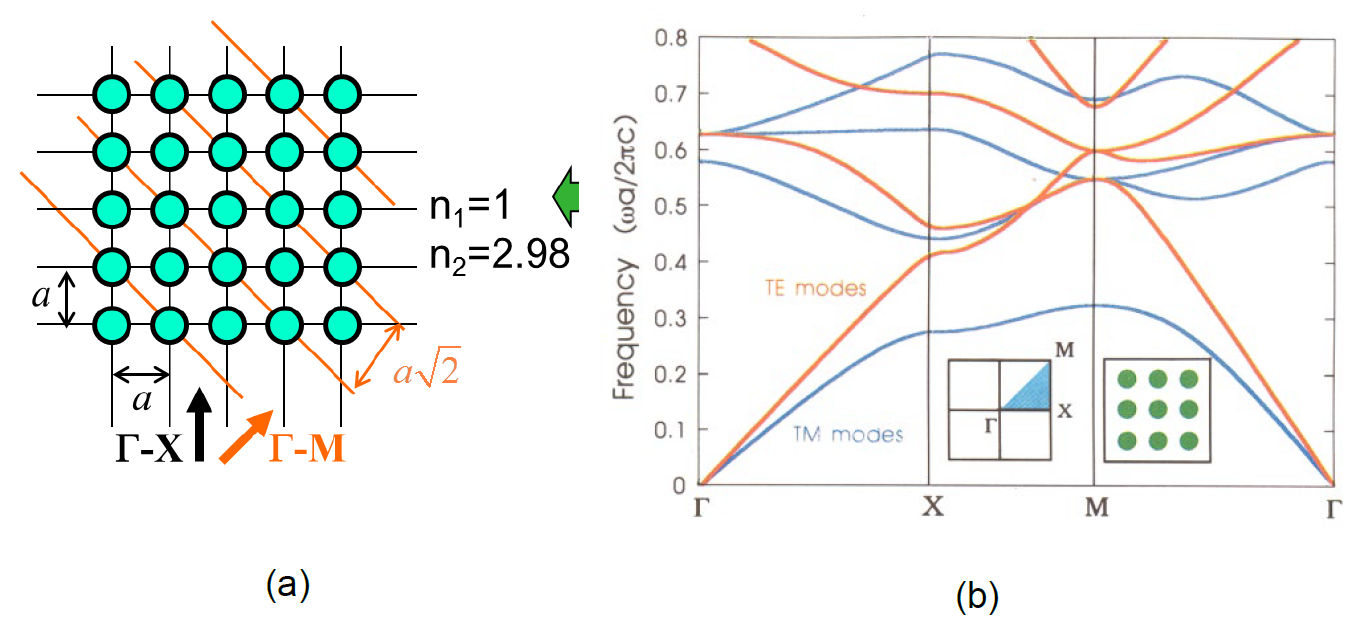
\includegraphics[width=0.95\textwidth]{fig1.png}
    \caption{(a) 2-D square lattice photonic crystal with pillars surrounded by air. The different k-directions are marked; (b) Band structure for the TE-modes and TM-modes. NOTE: Ratio radius of the pillar to period of the structure r/a = 0.2.}
    \label{fig:fig1}
\end{figure}

\begin{displayquote}
    \textbf{1.} Explain how the simulation file \verb|“square2D.fsp”| and the script \verb|“square2D.lsf”| calculate the band diagram for the TM-modes. Explain step by step how they work, how they are interconnected and how what they do relate with the methodology that we saw in the lecture for the calculation of the band diagrams.
\end{displayquote}
The results of the simulation are presented on Figure~\ref{fig:TM}. 
\verb|“square2D.fsp”| contains the setup for the simulation. Geometry of the PC and its material is defined by the circles in the structure group \verb|rect_pc|. The solver box FDTD contains one unit cell of the PC, and sets the Bloch boundary conditions for 2D simulation. There is a randomly positioned array of dipoles to excite all possible modes in the PC, as well as randomly positioned array of time monitors to record the electric field inside. 

There are three sweeps for $\Gamma$-X-M-$\Gamma$ range of directions of k-vector components varying from 0 to 0.5 in corresponding order.  

The script \verb|“square2D.lsf”| initiates three parameter sweeps for x- and y-components of the Bloch vector in FDTD. During the sweep, E(t) is added up for all time monitors. The resonances are then found and recorded. The script fills up the matrix \verb|fs_all| consecutively with the results of the sweeps, then normalizes it with the PC period, transposes this matrix and plots the data points against the frequency. 
\begin{figure}[ht]
   \centering
    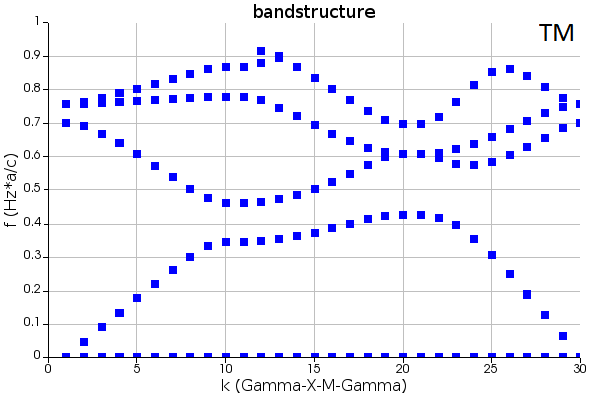
\includegraphics[width=0.75\textwidth]{electric_dipole.png}
    \caption{Band diagram for TM-modes}
    \label{fig:TM}
\end{figure}
\begin{figure}[ht]
   \centering
    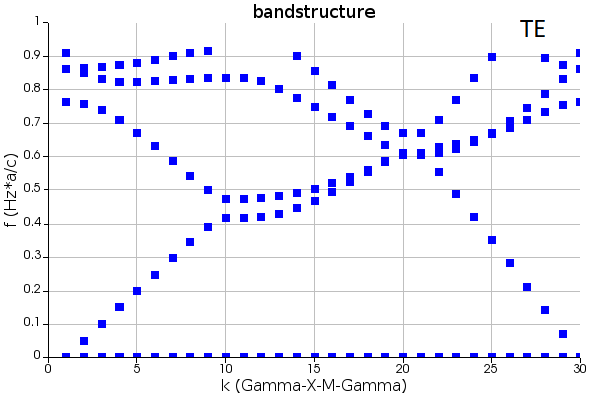
\includegraphics[width=0.75\textwidth]{magnetic_dipole.png}
    \caption{Band diagram for TE-modes}
    \label{fig:TE}
\end{figure}
\begin{displayquote}
    \textbf{2.} Calculate the band diagram for the same structure for TE-modes. What, if anything, do you need to change?
\end{displayquote}

The results of the simulation are presented on Figure~\ref{fig:TE}. 
In this script, \verb|Electric dipole| stands for TM- and \verb|Magnetic dipole| for TE-modes. In order to change polarization, the string variable \verb|dipole type| of \verb|dipole_cloud| has to be changed to desired one. This sets the corresponding variable in the script which generates the random array of dipoles. 

\begin{displayquote}
    \textbf{3.} Now, modify the script to calculate the band diagram for both TE-modes and TM-modes of the 2-D square lattice that we saw in the lecture and it is copied below:
\end{displayquote}

Notice that you will need to do the following changes: 
\begin{itemize}
    \item Pillars material is now a high index dielectric, with $\varepsilon=8.9$. 
    \item Ratio r/a = 0.2.  
\end{itemize}

The results of the simulation are presented on Figure~\ref{fig:tm-te}. 
\begin{figure}[ht]
   \centering
    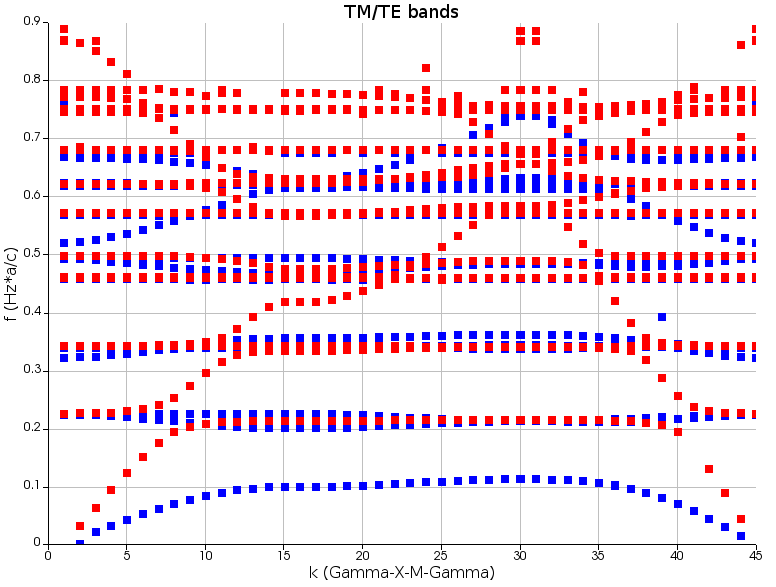
\includegraphics[width=0.75\textwidth]{tm-te.png}
    \caption{Band diagram for TM-modes (blue) and TE-modes (red).}
    \label{fig:tm-te}
\end{figure}
Index of the material of the dielectric can be changed in \verb|Structure Group| variables. Ratio r/a can be set by either changing the period of the structure or the radius of the pillar variables. In the original file, the period is set to 500 nm and the radius is 120 nm, r/a = 0.24, which makes it convenient to simply change the radius to 100 nm so that r/a = 0.2. 

To switch between the polarizations, a command can be used: \\ 
\verb|setnamed("dipole_cloud", "dipole type", "Electric/Magnetic dipole");|

Both plots can in principle be drawn on the same graph by using \verb|holdon;|, and distinguishing them by setting different colors \verb|"plot points, color=red/blue"|. 

\begin{displayquote}
    \textbf{a.} Calculate the band diagram for both TE and TM modes. Plot the band diagram using normalized frequency units: $f_{norm} = k * a / (2 * \pi * c)$ and normalized k vectors: $k_{norm} = k * a / (2 * \pi)$. Use 15 values of k in each side of the reduced Brillouin zone. What do you need to modify in the script? 
\end{displayquote}
Call number of k vectors \verb|nk|. Number of wavevectors in our model is the number of points in each sweep, for example, \verb|setsweep("Gamma-X","Number of points",nk);| Besides that, the matrix which accumulates the results has to be large enough to include all wavevectors for all sweeps. Pasting the results in this matrix also has to be in accordance with the assigned number of wavevectors per sweep. Finally, plotting the results should include all of k-values. 
\begin{displayquote}
    \textbf{b.} Try to find 15 bands instead of 10. What do you need to modify in the script? 
\end{displayquote}
Call number of bands \verb|nb|. The script is looking for 50 bands by default. Using \\ \verb|fs_all(1:nb,1:nk)= resonance.fs(1:nb,1:nk);| \\ we can change the number of bands in the results. 
\begin{displayquote}
    \textbf{c.} In the band diagram, indicate where the different Brillouin zone regions start and end: k values ($k_x$ and $k_y$ components) corresponding to $\Gamma$, X and M.
\end{displayquote}
The results are presented on Figure~\ref{fig:points}. 

\begin{figure}[ht]
   \centering
    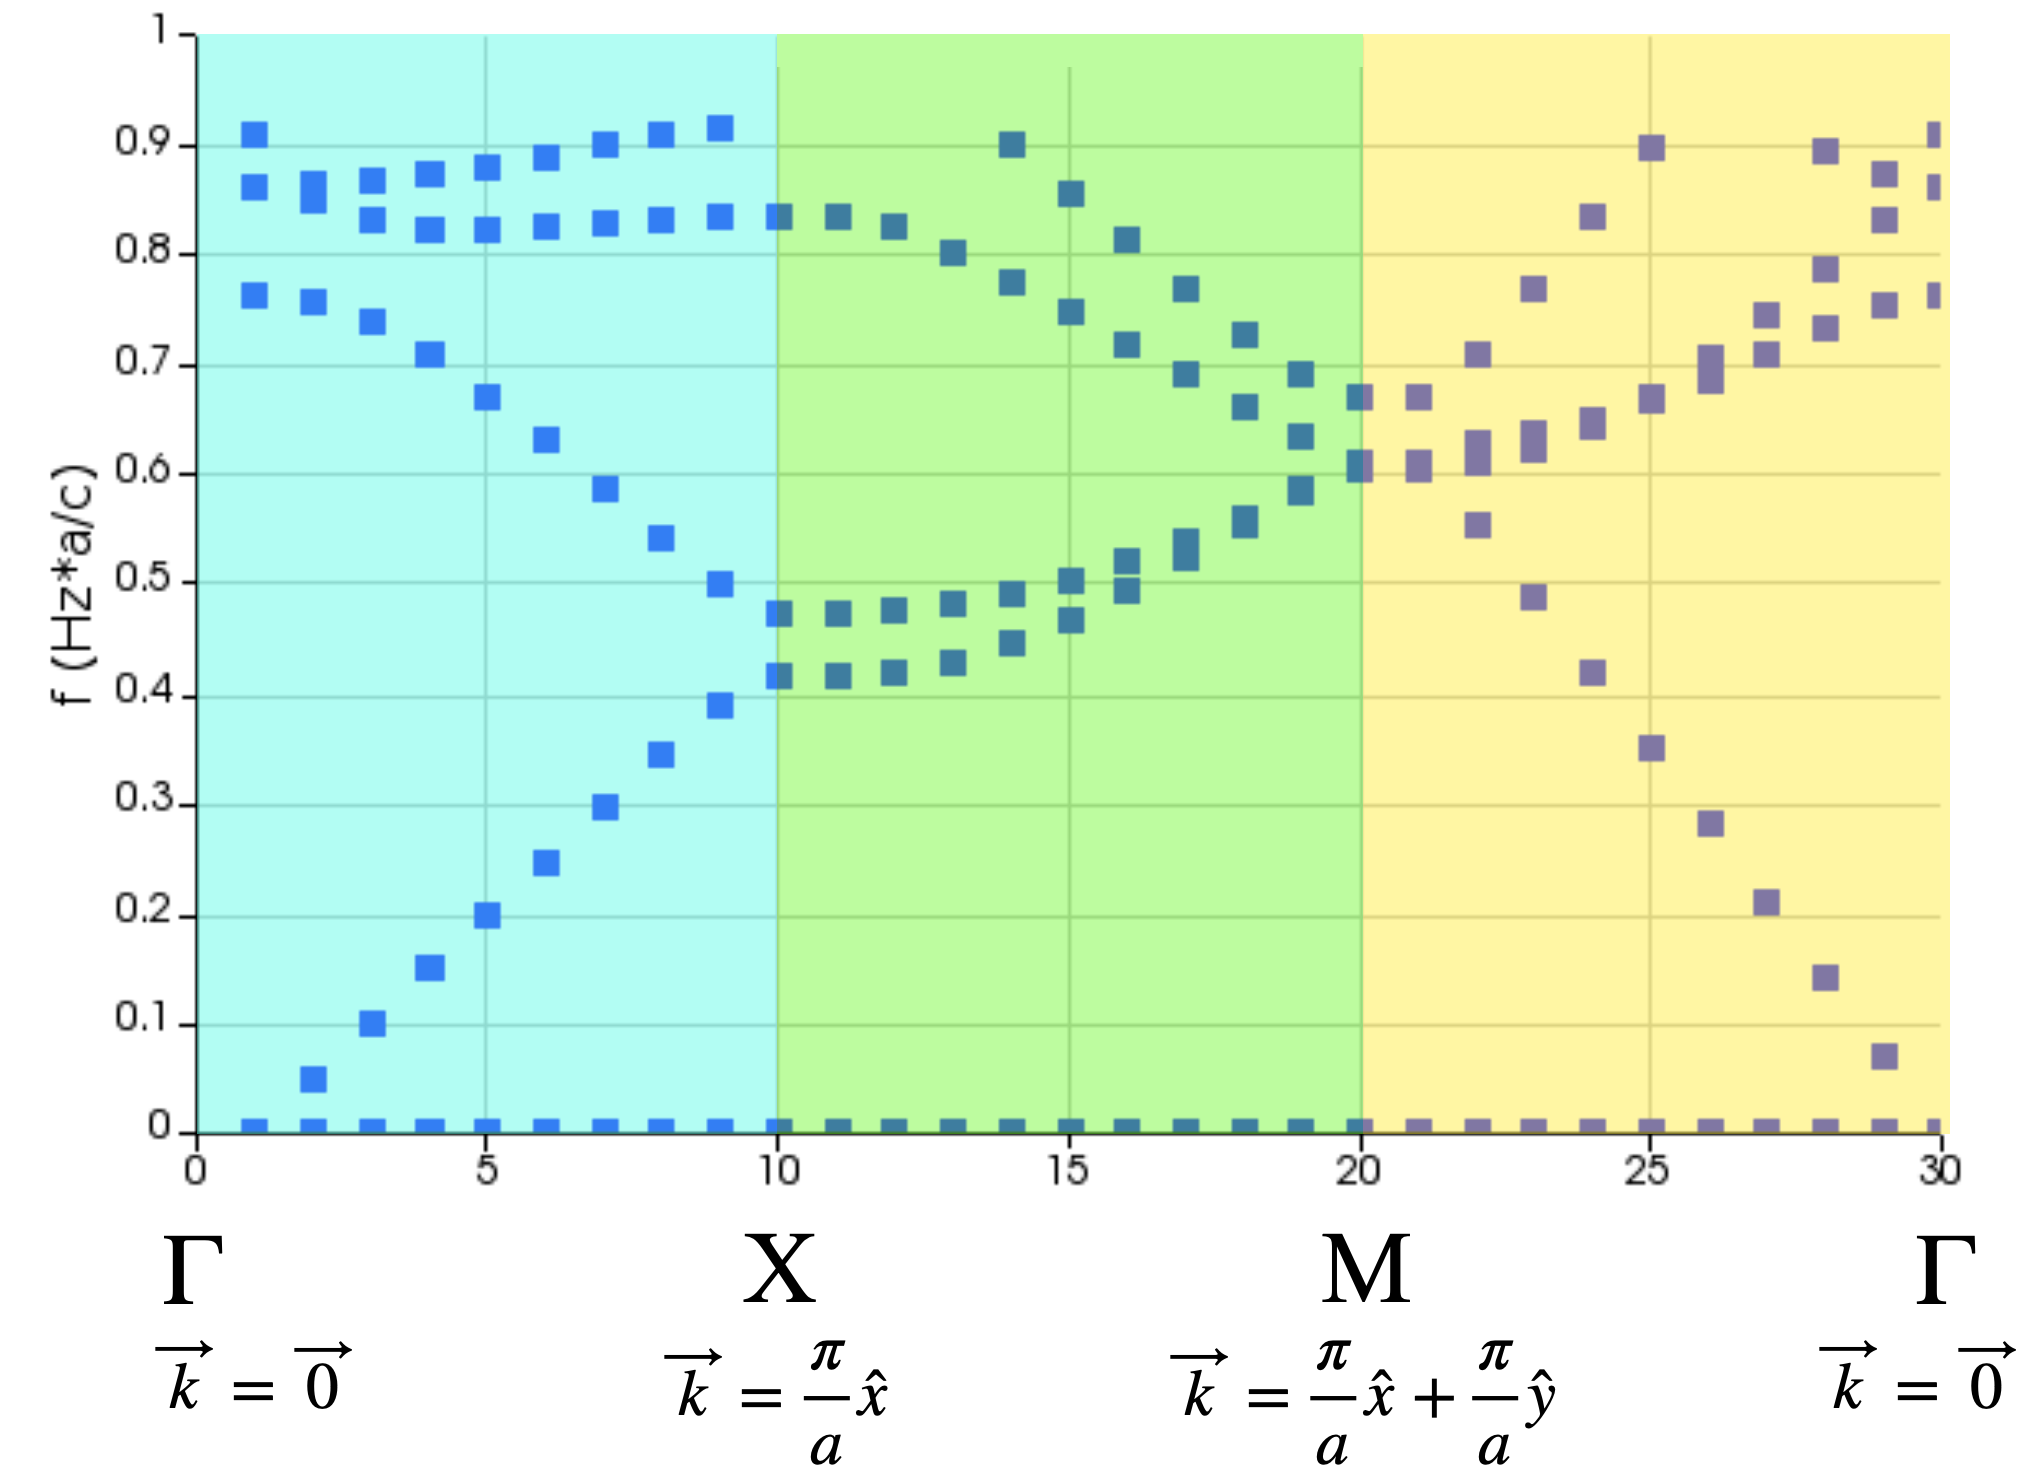
\includegraphics[width=0.75\textwidth]{points.png}
    \caption{Band diagram with Brillouin zone regions and k values corresponding to $\Gamma$, X and M points.}
    \label{fig:points}
\end{figure}

\begin{displayquote}
    \textbf{4.} Explain how you choose the ranges of k-vectors to be used in the sweeps. Note that you need to indicate which sweeps you want to make on the “Optimization and Sweep” tab.
\end{displayquote}


A number of k-vectors (10 or 15) is set along the irreducible Brillouin zone between the critical points. In our case (Figure~2, b) we consider $\Gamma: \; \vec{k}=\Vec{0}$, X: $\; \vec{k}= \frac{\pi}{a}\hat{x} $, and M: $\; \vec{k}=\frac{\pi}{a}\hat{x}+ \frac{\pi}{a}\hat{y}$. Normalization by $\nicefrac{2 \pi}{a}$ leads to changing the multipliers of unit vectors to $\nicefrac{1}{2}$. Hence for the sweep $\Gamma$-X, we run $\vec{k}=0\hat{x}+0\hat{y} \rightarrow \vec{k}=0.5\hat{x}+0\hat{y}$, for X-M we run $\vec{k}=0.5\hat{x}+0\hat{y} \rightarrow \vec{k}=0.5\hat{x}+0.5\hat{y}$, and, finally, for M-$\Gamma$ $\vec{k}=0.5\hat{x}+0.5\hat{y} \rightarrow \vec{k}=0\hat{x}+0\hat{y}$. The sweep variables are \verb|::model::kx/ky| correspondingly.

\begin{displayquote}
    \textbf{5.} Modify now the Lumerical model to simulate an inverse structure (a dielectric block with $\varepsilon$ = 11.4 with air circular holes perforated in it).
Inspiring yourself on the “Gap maps” shown in the Figure below, choose the correct ratio “r/a” to have bandgaps for both TE-modes and TM-modes. Calculate the bandstructure for TE-modes and TM-modes for the chosen “r/a”.
\end{displayquote}

\begin{figure}[ht]
   \centering
    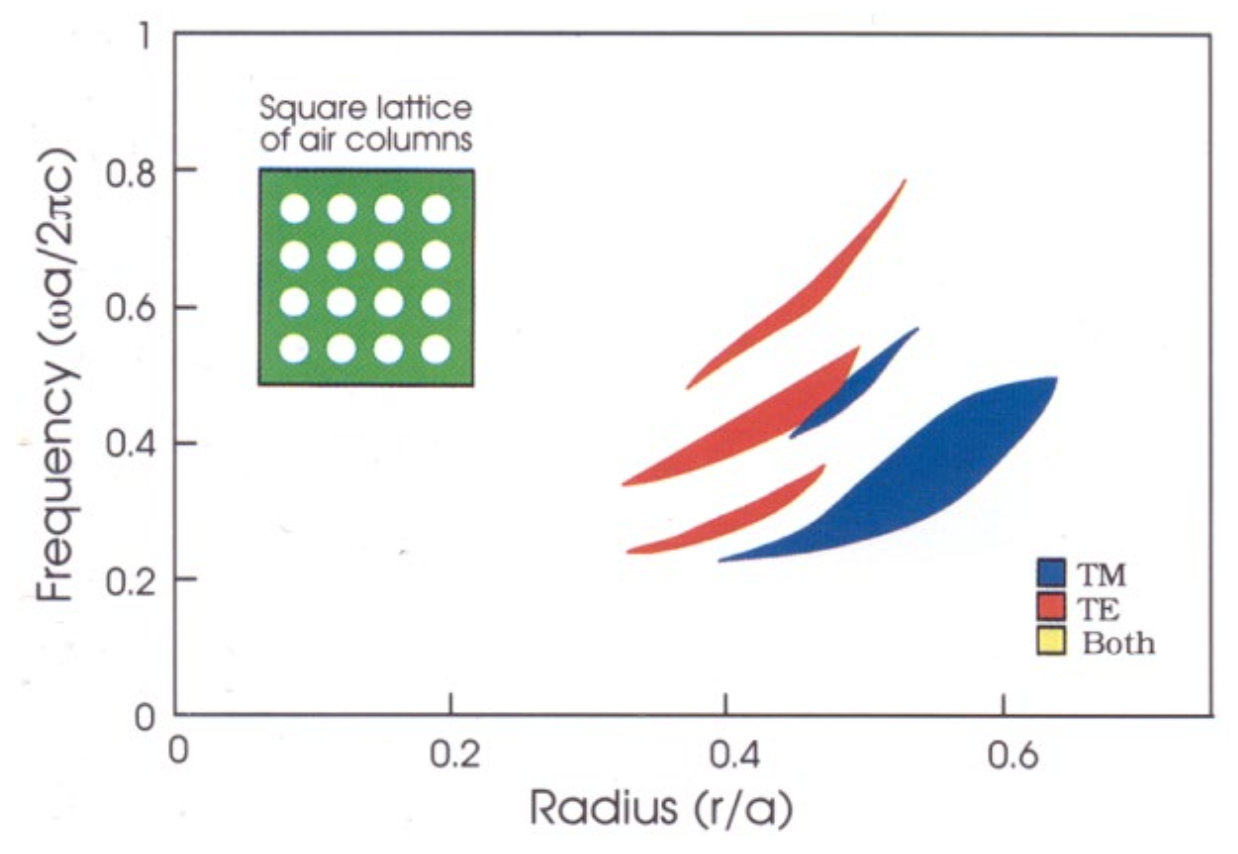
\includegraphics[width=0.75\textwidth]{fig3.png}
    \caption{Gap maps corresponding to a 2-D square lattice of air holes in dielectric ($\varepsilon$ = 11.4).The red and blue regions show the range of normalized frequencies for which there is a bandgap for each value of normalized radius (r/a).}
    \label{fig:fig3}
\end{figure}


For simplicity, we can change FDTD solver box background index to 11.4 and set the circle index to 1. It looks like the intersection of blue and red zones occurs at r/a $\approx$ 0.45. To match it, we can set r = 225 nm. 

The results can be seen in Figure~\ref{fig:q5}. There indeed is a bandgap in both TM and TE polarizations, although such large radius in relation to size of solver box may challenge the accuracy of the results: the chance that the time monitor finds itself outside of the circle is now lower. The results are the same for the case if the dielectric is represented not by the background index but by an additional body with the same index. 

\begin{figure}[ht]
   \centering
    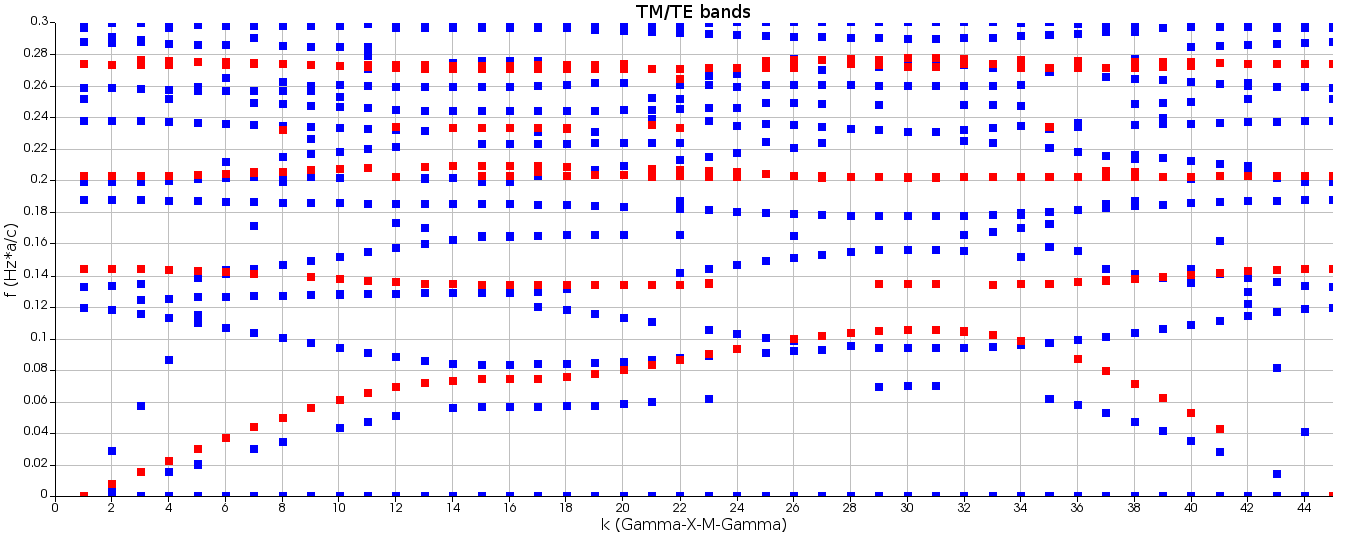
\includegraphics[width=0.95\textwidth]{q5.png}
    \caption{Band diagram corresponding to a 2-D square lattice of air holes in dielectric ($\varepsilon$ = 11.4, r/a = 0.45) with TM-modes (blue) and TE-modes (red).}
    \label{fig:q5}
\end{figure}


\end{document}
